\subsection{Architectural Views}

\subsubsection{Logical View}

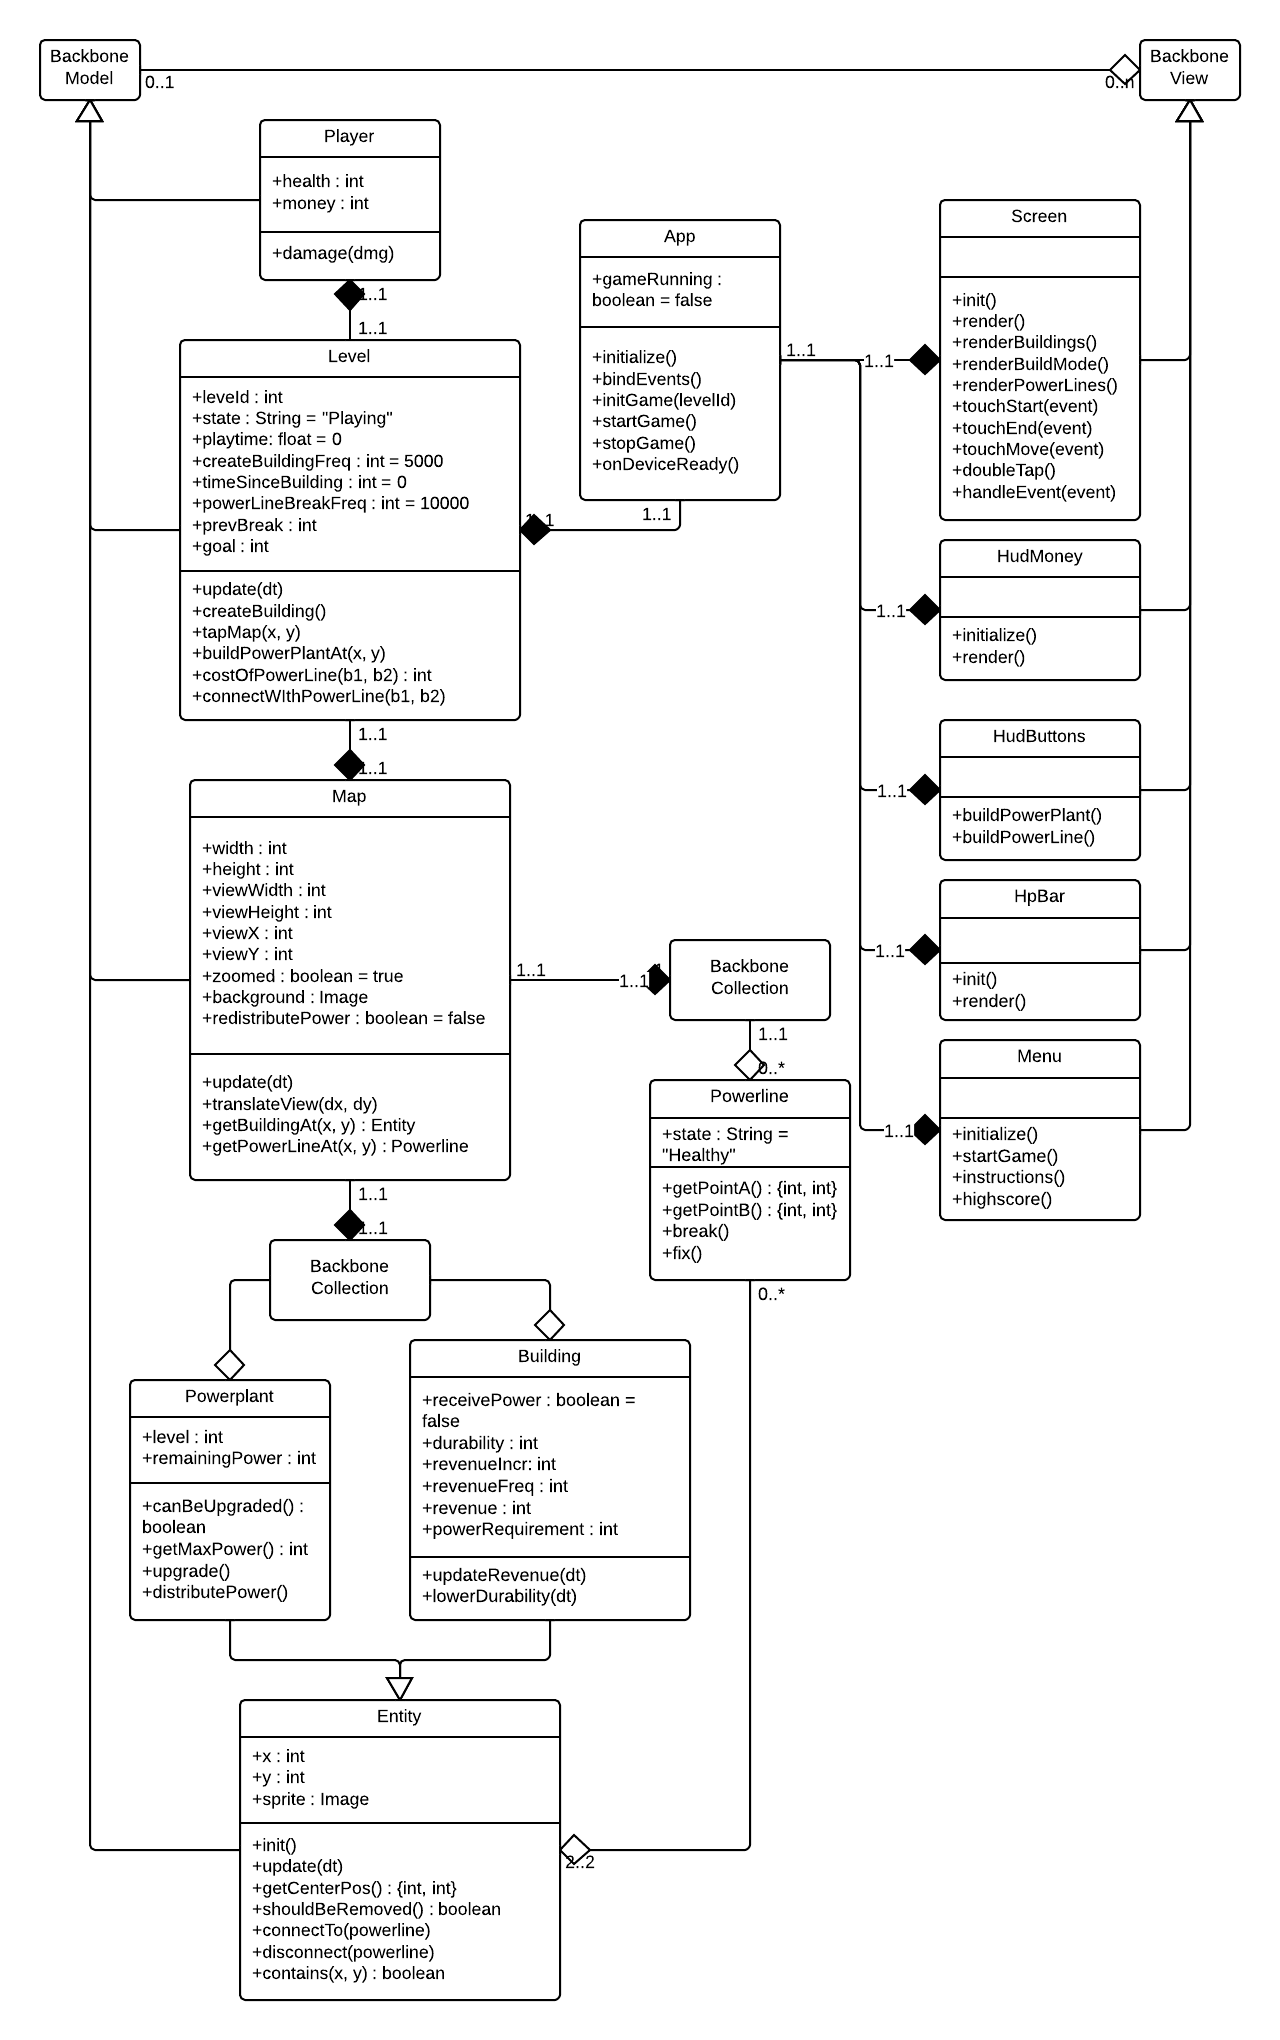
\includegraphics[width=\textwidth]{pictures/class_diagram}

\subsubsection{Process View}

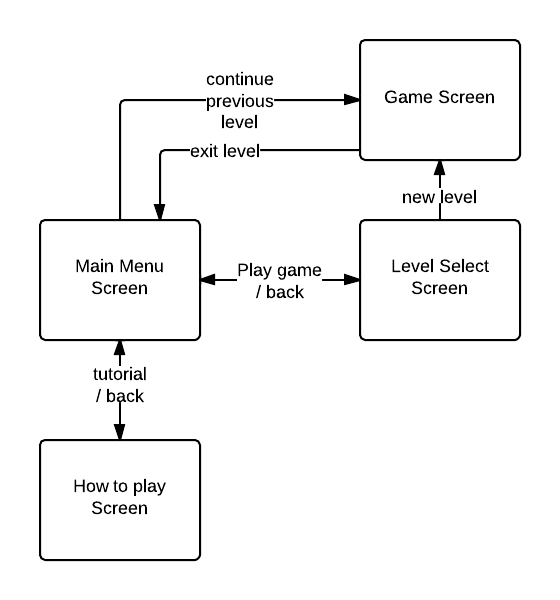
\includegraphics[width=\textwidth]{pictures/process_view_screen_flow}

The main menu screen is the entry point for the game. From there you can go to the "How to Play" screen, 
to read about how the game works. You can go to the "Level Select" screen to start a new level, or load the 
most recent level and continue playing from where you last left of. While playing you can exit the current 
level and return to the main menu.

\subsubsection{Physical View}

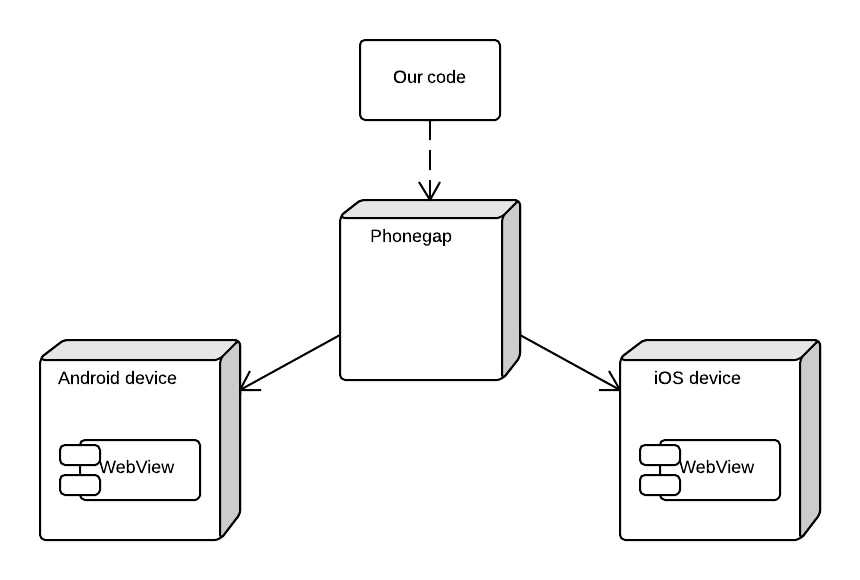
\includegraphics[width=\textwidth]{pictures/deployment_diagram}
%Add figure text, deployment diagram

\subsubsection{Development View}

The development view is separated into hierarchically into layers. The first layer is the game state 
and logic layer. The Models store the current state of the game which gets updated by the game loop 
and input from the player. The second layer decides how the game state is to be presented to the 
player, this layer also receives user input from layer three which updates the game state. The third 
layer is the HTML code which handles the layout of the user interface and sends user input to the
second layer.

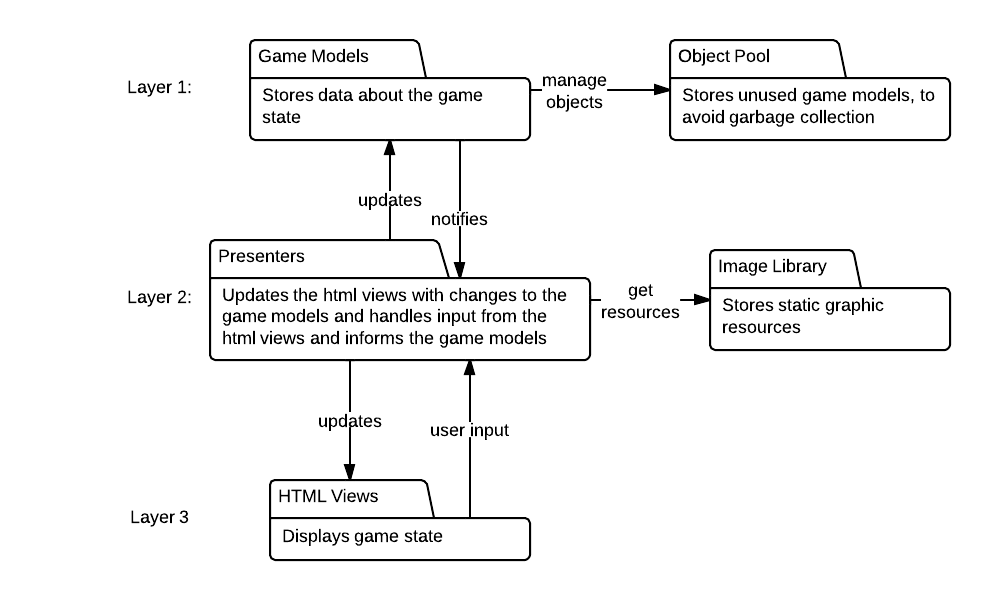
\includegraphics[width=\textwidth]{pictures/development_view}
